%% H2H4 Topology 

\documentclass[tikz,margin=2mm]{standalone}
\usepackage{amssymb}


\begin{document}

\tikzstyle{every node}=[fill=white,rectangle,rounded corners,inner sep=2,outer sep=0]

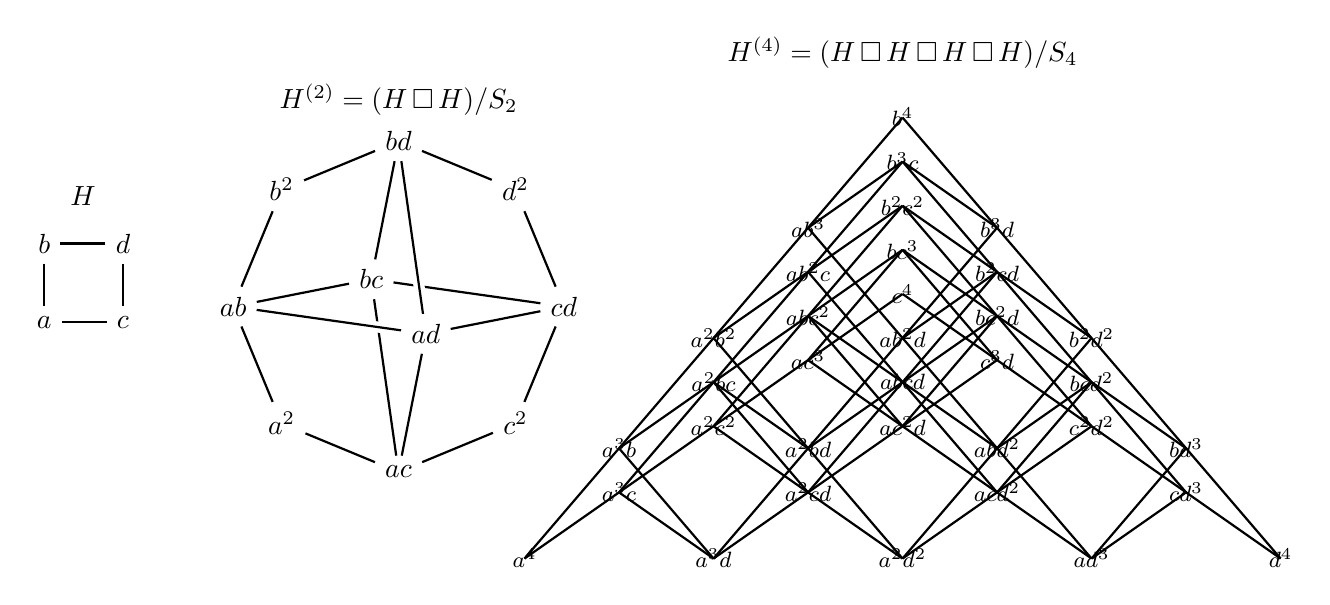
\begin{tikzpicture}[scale=1,style=thick,shorten >=0pt,shorten <=0pt]
 
\begin{scope}[xshift=-4.5cm,yshift=1.5cm,node distance=1cm]
\node (LRA) {$b$};
\node[below of = LRA] (RA) {$a$};
\draw [thick] (LRA) to  (RA);
\node[right of = RA] (RAG) {$c$};
\draw [thick] (RA) to  (RAG);
\node[right of = LRA] (LRAG) {$d$};
\draw [thick] (LRAG) to (LRA);
\draw [thick] (RAG) to  (LRAG);
\path (LRA) to node[above,yshift=10pt] {$H$} (LRAG);
\end{scope}
 
\begin{scope}[yshift=0.7cm,scale=0.7,shorten >=0pt,shorten <=0pt]
\coordinate (title) at (90:3.75); 
\draw (title) node {$H^{(2)}=(H\,\Box\, H)/S_2$};
%\draw (title) node {$H^{(2)}$:};
\draw (0:3) node[] (cd) {$cd$};  
\draw (45:3) node[] (d2) {$d^2$};  
\draw (90:3) node[] (bd) {$bd$};  
\draw (135:3) node[] (b2) {$b^2$};  
\draw (180:3) node[] (ab) {$ab$};  
\draw (225:3) node[] (a2) {$a^2$};  
\draw (270:3) node[] (ac) {$ac$};  
\draw (315:3) node[] (c2) {$c^2$};  
\draw (315:0.7) node[] (ad) {$ad$}; 
\draw (135:0.7) node[] (bc) {$bc$}; 
\draw[thick] (a2) -- (ab);  
\draw[thick] (ab) -- (b2);  
\draw[thick] (b2) -- (bd);  
\draw[thick] (bd) -- (d2);  
\draw[thick] (d2) -- (cd);  
\draw[thick] (cd) -- (c2);   
\draw[thick] (c2) -- (ac); 
\draw[thick] (ac) -- (a2); 
\draw[thick] (bc) -- (bd);   

\draw[thick] (ad) -- (ac); 
\draw[thick] (ac) -- (bc); 
\draw[thick] (ab) -- (bc);   
\draw[thick] (bc)-- (cd); 
\draw[thick] (cd) -- (ad); 
\draw[thick] (ad)-- (ab); 
\draw[line width=4pt,white] (bd) -- (ad);  \draw[thick] (bd) -- (ad); 
\draw[line width=4pt,,white] (ad)-- (ab);  \draw[thick] (ad)-- (ab); 
\end{scope}


\begin{scope}[xshift=1.6cm,yshift=-2.5cm,xscale=1.2,yscale=1.4,font=\footnotesize,thick] 
 

\coordinate (a4) at (0,0);
\coordinate (a3b) at (1,1);
\coordinate (a2b2) at (2,2);
\coordinate (ab3) at (3,3);
\coordinate (b4) at (4,4);

\coordinate (a3d) at (2,0);
\coordinate (a2bd) at (3,1);
\coordinate (ab2d) at (4,2);
\coordinate (b3d) at (5,3);
 
\coordinate (a2d2) at (4,0);
\coordinate (abd2) at (5,1);
\coordinate (b2d2) at (6,2);

\coordinate (ad3) at (6,0);
\coordinate (bd3) at (7,1);

\coordinate (d4) at (8,0);

\begin{scope}[yshift=-0.4cm]
\coordinate (a3c) at (1,1);
\coordinate (a2bc) at (2,2);
\coordinate (ab2c) at (3,3);
\coordinate (b3c) at (4,4);

\coordinate (a2cd) at (3,1);
\coordinate (abcd) at (4,2);
\coordinate (b2cd) at (5,3);
 
\coordinate (acd2) at (5,1);
\coordinate (bcd2) at (6,2);

\coordinate (cd3) at (7,1);
\end{scope}

\begin{scope}[yshift=-0.8cm]
\coordinate (a2c2) at (2,2);
\coordinate (abc2) at (3,3);
\coordinate (b2c2) at (4,4);

\coordinate (ac2d) at (4,2);
\coordinate (bc2d) at (5,3);

\coordinate (c2d2) at (6,2);
\end{scope}

\begin{scope}[yshift=-1.2cm]
\coordinate (ac3) at (3,3);
\coordinate (bc3) at (4,4);

\coordinate (c3d) at (5,3);
\end{scope}

\begin{scope}[yshift=-1.6cm]
\coordinate (c4) at (4,4);
\end{scope}


\draw (a4) to (a3b);
\draw (a3b) to (a2b2);
\draw (a2b2) to (ab3);
\draw (ab3) to (b4);

\draw (a3d) to (a2bd);
\draw (a2bd) to (ab2d);
\draw (ab2d) to (b3d);
 
\draw (a2d2) to (abd2);
\draw (abd2) to (b2d2);
 
\draw (ad3) to (bd3);
 
\draw (b4) to (b3d);
\draw (b3d) to (b2d2);
\draw (b2d2) to (bd3);
\draw (bd3) to (d4);

\draw (ab3) to (ab2d);
\draw (ab2d) to (abd2);
\draw (abd2) to (ad3);
 
\draw (a2b2) to (a2bd);
\draw (a2bd) to (a2d2);
 
\draw (a3b) to (a3d);

%% shift bc

\draw (a3c) to (a2bc);
\draw (a2bc) to (ab2c);
\draw (ab2c) to (b3c);

\draw (a2cd) to (abcd);
\draw (abcd) to (b2cd);
 
\draw (acd2) to (bcd2);
 
\draw (b3c) to (b2cd);
\draw (b2cd) to (bcd2);
\draw (bcd2) to (cd3);

\draw (ab2c) to (abcd);
\draw (abcd) to (acd2);
 
\draw (a2bc) to (a2cd);

%% shift bc

\draw (a2c2) to (abc2);
\draw (abc2) to (b2c2);

\draw (ac2d) to (bc2d);
 
\draw (b2c2) to (bc2d);
\draw (bc2d) to (c2d2);

\draw (abc2) to (ac2d);

%% shift bc

\draw (ac3) to (bc3);
\draw (bc3) to (c3d);

%%%%

\draw (ab3) to (b3c);
\draw (b3c) to (b3d);

\draw (ab2c) to (b2c2);
\draw (b2c2) to (b2cd);
\draw (a2b2) to (ab2c);
\draw (b2d2) to (b2cd); 

\draw (abc2) to (bc3);
\draw (bc3) to (bc2d);
\draw (a2bc) to (abc2);
\draw (bcd2) to (bc2d); 
\draw (a2bc) to (a3b);
\draw (bcd2) to (bd3); 

\draw (ac3) to (c4);
\draw (c4) to (c3d);
\draw (a2c2) to (ac3);
\draw (c2d2) to (c3d); 
\draw (a2c2) to (a3c);
\draw (c2d2) to (cd3); 
\draw (a4) to (a3c);
\draw (d4) to (cd3);

\draw (a3d) to (a2cd);
\draw (a2cd) to (ac2d);
\draw (ac2d) to (c3d);

\draw (a2d2) to (acd2);
\draw (acd2) to (c2d2);

\draw (ad3) to (cd3);

\draw (a3c) to (a3d);

\draw (a2c2) to (a2cd);
\draw (a2cd) to (a2d2);

\draw (ac3) to (ac2d);
\draw (ac2d) to (acd2);

\draw (a2bc) to (a2bd);

\draw (abc2) to (abcd);
\draw (abcd) to (abd2);
 
\draw (acd2) to (ad3);
  
\draw (abd2) to (bcd2);

\draw (a2bd) to (abcd);
\draw (abcd) to (bc2d);

\draw (ab2d) to (b2cd);

\draw (a4) node {$a^4$};
\draw (a3b) node {$a^3b$};
\draw (a2b2) node {$a^2b^2$};
\draw (ab3) node {$ab^3$};
\draw (b4) node {$b^4$};

\draw (a3d) node {$a^3d$};
\draw (a2bd) node {$a^2bd$};
\draw (ab2d) node {$ab^2d$};
\draw (b3d) node {$b^3d$};
 
\draw (a2d2) node {$a^2d^2$};
\draw (abd2) node {$abd^2$};
\draw (b2d2) node {$b^2d^2$};
  
\draw (ad3) node {$ad^3$};
\draw (bd3) node {$bd^3$};
 
\draw (d4) node {$d^4$};

\draw (a3c) node {$a^3c$};
\draw (a2bc) node {$a^2bc$};
\draw (ab2c) node {$ab^2c$};
\draw (b3c) node {$b^3c$};

\draw (a2cd) node {$a^2cd$};
\draw (abcd) node {$abcd$};
\draw (b2cd) node {$b^2cd$};
 
\draw (acd2) node {$acd^2$};
\draw (bcd2) node {$bcd^2$};
  
\draw (cd3) node {$cd^3$};
 
\draw (a2c2) node {$a^2c^2$};
\draw (abc2) node {$abc^2$};
\draw (b2c2) node {$b^2c^2$};

\draw (ac2d) node {$ac^2d$};
\draw (bc2d) node {$bc^2d$};
 
\draw (c2d2) node {$c^2d^2$};
  
\draw (ac3) node {$ac^3$};
\draw (bc3) node {$bc^3$};

\draw (c3d) node {$c^3d$};
 
\draw (c4) node {$c^4$};
 
%\node [left of=ab3,xshift=0cm,yshift=1cm,fill=none,rectangle,font=\normalsize] {$H^{(4)}$:};
\node [above of=b4,yshift=-5pt,fill=none,rectangle,font=\normalsize] {$H^{(4)}=(H\,\Box\, H \,\Box\, H \,\Box\,  H)/S_4$};

\end{scope} 

\end{tikzpicture}

\end{document}  